\documentclass[12pt]{article}

\title{Developement of a neural network framework in C++ and application to a particle physics dataset}
\author{Simone Balducci}
\date{}

\usepackage[hidelinks]{hyperref}
\usepackage{amsmath}
\usepackage{amsfonts}
\usepackage{amssymb}
\usepackage{amsthm}
\usepackage{bbold}
\usepackage[margin=2.8cm]{geometry}
\usepackage{pgfplots}
\usepackage{fancyhdr}
\usepackage{physics}
\usepackage{systeme,mathtools}
\usepackage{graphicx}
\usepackage{float}
\usepackage{relsize}
\usepackage{dsfont}
\usepackage{calligra}
\usepackage{float}
\usepackage[utf8]{inputenc}
\usepackage{tikz}
\usetikzlibrary{positioning}
\usepackage{listings}
\usepackage{xcolor}
\usepackage[backend=biber]{biblatex}
\addbibresource{biblio.bib}

\definecolor{codegreen}{rgb}{0,0.6,0}
\definecolor{codegray}{rgb}{0.5,0.5,0.5}
\definecolor{codepurple}{rgb}{0.58,0,0.82}
\definecolor{backcolour}{rgb}{0.95,0.95,0.92}

\lstdefinestyle{mystyle}{
    backgroundcolor=\color{backcolour},   
    commentstyle=\color{codegreen},
    keywordstyle=\color{blue},
    numberstyle=\tiny\color{codegray},
    stringstyle=\color{codepurple},
    basicstyle=\ttfamily\scriptsize,
    breakatwhitespace=false,         
    breaklines=true,                 
    captionpos=b,                    
    keepspaces=true,                 
	columns=flexible,
    numbers=left,                    
    numbersep=5pt,                  
    showspaces=false,                
    showstringspaces=false,
    showtabs=false,                  
    tabsize=2
}

\lstset{style=mystyle}


\newcommand{\vv}{\vec{v}}
\newcommand{\vw}{\vec{w}}
\newcommand{\vx}{\vec{x}}
\newcommand{\R}{\Re}
\newcommand{\la}{\lambda}
\newcommand{\lang}{\left\langle}
\newcommand{\rang}{\right\rangle}
\newcommand{\lbra}{\left\lbrace}
\newcommand{\rbra}{\right\rbrace}
\newcommand{\ih}{\hat{i}}
\newcommand{\jh}{\hat{j}}
\newcommand{\kh}{\hat{k}}
\newcommand{\nnabla}{\vec{\nabla}}
\newcommand{\rita}{\rightarrow}

\begin{document}

\maketitle
\begin{center}
	\url{https://github.com/sbaldu/Neural_network_HEP}
\end{center}

\begin{abstract}
  \noindent Nowadays neural networks are widely used in many branches of physics, in par\-ti\-cu\-lar 
  in particle physics. \\
  The Higgs ML challenge \cite{HiggsML} asked to classify in signal and background a set of events simulated based on the 
  ATLAS detector. This is exactly the kind of problem that could be effectively tackled using a neural 
  network. \\ \\
  Nowadays there are a lot of libraries already written to work with neural networks. The first two that
  come to mind, and also the largest ones, are Tensorflow \cite{TensorFlow} and PyTorch \cite{Pytorch}, which are available in Python, C++ 
  and other languages. \\
  These libraries are very thoroughly written and efficient, but from an accademic point of view it is
  instructive, in order to really understand the functioning of neural networks, to learn how to write 
  them from scratch. \\ \\
  The goal of this project is to write from scratch in C++ a framework for wor\-king with neu\-ral networks, 
  test it with the MNIST \cite{MNIST} dataset and finally use it to tackle the Higgs ML challenge.
\end{abstract}
\pagebreak

\tableofcontents
\vspace{1cm}
\lstlistoflistings
\pagebreak

\section{Physical background}
\subsection{Review of special relativity}
The most fundamental equation in special relativity defines the 4-momentum of a particle:
\begin{equation}
  E^2 = p^2c^2 + m^2c^4
\label{fundamental}
\end{equation}
where $E$ is the energy of the particle, $p$ is its momentum, $m$ is the rest mass and $c$ is the speed of 
light. \\
In particle physics usually the following units are used:
\begin{itemize}
  \item Energy is measured in $GeV$, where $1\,eV$ is the energy acquired by an electron accelerated by an
	electric potential of $1\,V$ over a distance of $1\,m$.
  \item Momentum is measured in $GeV/c$
  \item Mass is measured in $GeV/c^2$
\end{itemize}
It should be noted that usually, for convenience, the units of mass, momentum and energy are all indicated 
simply as $GeV$. \\
When using this units, Eq. \ref{fundamental} assumes the convenient form:
\begin{equation}
  E^2 = p^2 + m^2
  \label{fundamental_conv}
\end{equation}
The relativistic momentum is defined as:
\begin{equation}
  p = \gamma m v
\end{equation}
where $\gamma m$ is the relativistic mass, and $\gamma$ is a unitless constant known as the Lorentz factor
and defined as:
\begin{equation}
  \gamma = \frac{1}{\sqrt{1 - \beta^2}}
\end{equation}
where $\beta$ is $v/c$. \\
The kinematics of a particle is fully defined by the combination of its energy and the three components
of its momentum. These four quantities are known as the 4-momentum of the particle. \\ \\
The rest mass is an intrinsic property of a particle. To measure the mass of a particle we
need the 4-momenta of its products. \\
If a particle $H$ decays in two generic particles $A$ and $B$, by the conservation of energy and momentum
we can write:
$$
	E_H = E_A + E_B \hspace{2cm} \vec{p}_H = \vec{p}_A + \vec{p}_B
$$
The 4-momenta of both $A$ and $B$ are measured in the detector, which means that we can calculate the mass
of $H$ as:
\begin{equation}
  m_H = \sqrt{E^2_H - p^2_H}
\end{equation}
This quantity is called invariant mass, because it is always the same for all the possible combinations of
$E_H$ and $p_H$, at least in an ideal detector.

\subsection{Review of particle physics}
\begin{figure}
  \centering
  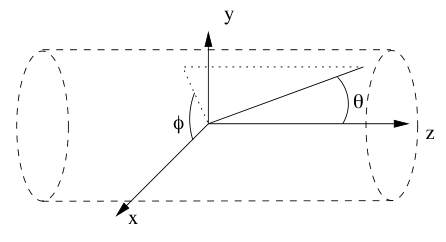
\includegraphics[scale=0.8]{img/atlas_frame.png}
  \caption{Reference frame used in the ATLAS experiment}
\end{figure}
In the conventional 3D reference frame used in the ATLAS experiment, the $z$ axis points along the horizontal 
beam line and the $x$ and $y$ axes are in the transverse plate, with the $y$ axis pointing towards the top 
of the detector. The angle $\theta$ is the polar angle and $\phi$ is the azimuthal angle. \\
Transverse quantities (mass, momentum and energy) are defined as projections on the $x-y$ plane. \\
Usually, instead of the polar angle $\theta$ it is useful to use the pseudorapidity $\eta$, which is defined
as:
\begin{equation}
  \eta = -\log \tan(\frac{\theta}{2})
\end{equation}
A pseudorapidity $\eta=0$ corresponds to a particle moving on the $x-y$ plane, whereas $\eta=\pm\infty$
corresponds to a particle traversing along the $z$ axis. \\
A practical difficulty is that many particles are lost in the direction of the $z$ axis, which means that we 
can count on conservation laws only on the transverse plane, thus the importance of defining transverse 
quantities. \\ \\
Now that we have described the spatial and angular coordinates used in this kind of experiments, we can 
define some other important quantities. \\
The components of momentum can be written as:
\begin{equation}
  \vec{p} = \begin{pmatrix}
	p_x \\
	p_y \\
	p_z
  \end{pmatrix} = \begin{pmatrix}
	p_T\cos\phi \\
	p_T\sin\phi \\
	p_T\sinh\eta
  \end{pmatrix}
\end{equation}
where $p_T$ is the transverse momentum, defined as
\begin{equation}
  p_T = \sqrt{p_x^2 + p_y^2}
\end{equation}
The missing transverse energy, $\vec{E}^{miss}_{T}$ is a two dimensional vector defined as:
\begin{equation}
  \vec{E}^{miss}_{T} = \begin{pmatrix}
	|\vec{E}^{miss}_{T}| \cos\phi_T \\
	|\vec{E}^{miss}_{T}| \sin\phi_T
  \end{pmatrix}
\end{equation}
where $\phi_T$ is the azimuthal angle of the missing transverse energy. \\
The invariant mass $m_{inv}$ of two particles is the invariant mass of the sum of the two 4-momenta, and 
the transverse mass $m_{tr}$ is the invariant mass of the sum of the two 4-momenta setting the $z$ component 
to zero, thus only keeping the transverse components.
So if $\vec{a}$ and $\vec{b}$ are the 4-momenta of two particles $A$ and $B$, $m_{inv}(\vec{a},\vec{b})$ 
and $m_{tr}(\vec{a},\vec{b})$, neglecting the two rest masses, are defined as:
\begin{equation}
  m_{inv}(\vec{a},\vec{b}) = \sqrt{\left(|\vec{a}| + |\vec{b}| \right)^2 
  - (a_x^2 + b_x^2)^2 - (a_y^2 + b_y^2)^2 - (a_z^2 + b_z^2)^2}
\end{equation}
\begin{equation}
  m_{tr}(\vec{a},\vec{b}) = \sqrt{\left(\sqrt{a_x^2 + a_y^2} + \sqrt{b_x^2 + b_y^2}\right)^2 
  - (a_x^2 + b_x^2)^2 - (a_y^2 + b_y^2)^2}
\end{equation}
where $|\vec{a}| = \sqrt{a_x^2 + a_y^2 + a_z^2}$. \\
The pseudorapidity separation between two particles $A$ and $B$ is defined as:
\begin{equation}
  |\eta_A - \eta_B|
\end{equation}
and their R separation is:
\begin{equation}
  \sqrt{(\eta_A - \eta_B)^2 + (\phi_A - \phi_B)^2}
\end{equation}

\subsection{Description of the dataset and goal of the project}
The Higgs boson dacays into two taus leptons. This process is theoretically interesting, becuase the Higgs 
boson is the particle responsible for the mass of the other elementary particles, but it is an experimentally 
challenging one. This difficulty is due to two reasons:
\begin{itemize}
  \item The neutrinos are not measured in the detector, so their presence in the final state makes it 
	difficult to evaluate the mass of the Higgs candidate
  \item The $Z$ boson can also decay in two tau leptons, and this process happens much more frequently than 
	the decay of the Higgs boson. Furthermore, since the masses of the $Z$ and $H$ bosons are very similar 
	(respectively $91\,GeV$ and $125\,GeV$), the two events are very difficult to separate.
\end{itemize}
The simulated data \cite{CERNOpenDataHiggsML} contains signal and background events. The signal events are those in which Higgs bosons
are produced. The background events are generated by other well known processes which can produce events with 
at least one electron or muon and a hadronic tau, thus mimicking the signal. For simplicity, only three
background processes are used:
\begin{itemize}
  \item Decay of $Z$ boson into two tau leptons
  \item Decay of a pair of $top$ quarks into a lepton and a hadronic tau
  \item Decay of the $W$ boson into an electron or muon and a hadronic tau
\end{itemize}
The particles and pseudo-particles of interest in this case are electrons, muons, hadronic tau, jets and 
missing transverse energy. \\
Electrons, muons and hadronic tau are the three leptons. Electrons and muons live long enough to reach the 
detector, so their 4-momenta can be measured directly. Taus, on the other hand, decay almost immediately 
into either an electron and two neutrinos, a muon and two neutrinos or a charged particles and a neutrino. \\
Jets are pseudo particles that originate from a high energy quark or gluon, and they appear in the detector 
as collimated energy deposits. \\ \\
The goal of the challenge is to classify each event as signal or background. Each entry of the dataset
contains $30$ features, in addition to the classification label, the event id and some weights to be used
in when calculating the score of the challenge. The last two are of no use for this project, so will be 
discarded in the preprocessing of the data. \\
The features are the measures of some primivite physical quantities of the particles, and others are more
complex quantities calculated from the privitive ones. \\
Here is a full list of the primitive features:
\begin{itemize}
  \item Transverse momentum of the hadronic tau
  \item pseudorapidity $\eta$ of the hadronic tau
  \item aximuth angle $\phi$ of the hadronic tau
  \item transverse momentum of the lepton
  \item pseudorapidity $\eta$ of the lepton
  \item aximuth angle $\phi$ of the lepton
  \item missing transverse energy
  \item aximuth angle $\phi$ of the missing transverse energy
  \item total transverse energy in the detector
  \item number of jets
  \item transverse momentum of the leading jet
  \item pseudorapidity $\eta$ of the leading jet
  \item aximuth angle $\phi$ of the leading jet
  \item transverse momentum of the subleading jet
  \item pseudorapidity $\eta$ of the subleading jet
  \item aximuth angle $\phi$ of the subleading jet
  \item scalar sum of the transverse momentum of all the jets
\end{itemize}
and the list of the derivate features:
\begin{itemize}
  \item estimated mass of the Higgs boson candidate
  \item transverse mass between the missing transverse energy and the lepton
  \item invariant mass of the hadronic tau and the lepton
  \item modulus of the vector sum of the transverse momentum of the hadronic tau, the lepton and the missing 
	transverse energy vector
  \item absolute value of the pseudorapidity separation between the two jets
  \item invariant mass of the two jets
  \item product of the pseudorapidities of the two jets
  \item $R$ separation between the hadronic tau and the lepton
  \item the modulus of the vector sum of the missing transverse momenta and the transverse momenta of the 
	hadronic tau, the lepton, the leading jet and the subleading jet
  \item the sum of the moduli of the transverse momenta of the hadronic tau, the lepton, the leading jet
	and the subleading jet and the other jets
  \item the ratio of the transverse momenta of the lepton and the hadronic tau
  \item the centrality of the azimuthal angle of the missing transverse energy vector with respect to the 
	hadronic tau and the lepton
  \item the centrality of the pseudorapidity of the lepton with respect to the two jets
\end{itemize}
\pagebreak

\section{Implementation of the neural network framework}
In this section is show the derivation of the backpropagation algorithm, which is used for training the 
neural network. \\
After that, the structure of the C++ code is described, in particular the implementation of the activation
functions, the loss function and the class for the neural network.
\subsection{Description of the error backpropagation algorithm}
We derive the backpropagation algorithm for a general network having a feed-forward topology, an 
arbitrary differentiable non-linear activation function and a class of error functions. \\
In a feed-forward network we have that each unit computes a weighted sum of its inputs as:
\begin{equation}
  a_j = \sum_i w_{ji}z_i
\end{equation}
where $z_i$ is the activated input. \\
The terms $a_j$ are then passed inside the activation function $h(\cdot)$, resulting in:
\begin{equation}
  z_j = h(a_j)
\end{equation}
Here $z_j$ could be the outputs of the network and $a_j$ could be the input. \\
This process is called \textit{forward propagation}, because there is a forward-directed flow of
information inside the network. \\
Now, to adjust the weights $w_{ji}$ we need to calculate the gradient of the terms of the error  
function, $E_n$. Since the value of the error only depends on the weights through terms $a_j$, we 
can use the chain rule:
\begin{equation}
  \frac{\partial E_n}{\partial w_{ji}} = 
  \frac{\partial E_n}{\partial a_{j}}\frac{\partial a_j}{\partial w_{ji}}
\end{equation}
where we see that the second derivative is simply $z_i$, and we call the first term $\delta_j$
\begin{equation}
  \delta_j = \frac{\partial E_n}{\partial a_j}
\end{equation}
So, we thus obtain the simple equation:
\begin{equation}
  \frac{\partial E_n}{\partial w_{ji}} = \delta_j z_i
  \label{loss_gradient_weight}
\end{equation}
This means that the problem of calculating the gradient of the error function boils down to
calculating $\delta_j$. \\
For the output layer it's trivial to calculate $\delta_j$, since it's simply:
\begin{equation}
  \delta_j = y_j - t_j
  \label{output_delta}
\end{equation}
where $t_j$ are the labels given in the training data. \\
For the hidden layers we use again the chain rule:
\begin{equation}
  \delta_j = \frac{\partial E_n}{\partial a_j}
  = \sum_k \frac{\partial E_n}{\partial a_k}\frac{\partial a_k}{\partial a_j}
  \label{hidden_layers_delta}
\end{equation}
where $\partial E_n / \partial a_k = \delta_k$ and $\partial a_k / \partial a_j = h'(a_j)w_{kj}$
so we obtain:
\begin{equation}
  \delta_j = h'(a_j)\sum_k w_{kj}\delta_k
  \label{simplified_hidden_layer_delta}
\end{equation}
So we see that the value of $\delta$ for a particular hidden unit can be obtained by propagating backwards 
the $\delta$ values from layers higher up in the network.

\subsection{Constructing the activation functions}
The choice of the activation function is of the highest importance when working with neural networks. \\
It is very convenient to write the activation functions as functors, instead of normal functions. This is
convinient because then the activation function can be passed to the neural network as a template parameter,
thus making it known at compile time. \\
A functor is an object that behaves like a function. In $C++$, functors are defined by declaring a struct 
and providing an operload for the $operator()$. These structs must be templated on the type of the data
contained in the neurons of the neural network. \\
As an example, below is reported the code of the most common and widely used activation function, the sigmoid
function, which is shown in Fig. \ref{sigmoid} and is mathematically defined as:
\begin{equation}
  S(x) = \frac{1}{1 + e^{-x}}
\end{equation}
\begin{figure}[H]
  \centering
  \begin{tikzpicture}[xscale=0.7, yscale=3.5]
  \draw[->] (-6, 0) -- (6, 0) node[right] {$x$};
  \draw[->] (0, -0.2) -- (0, 1.3) node[right] {$S(x)$};
  \draw (0, 1) node[anchor=south west] {$1$};
  \draw (0, 1) node {$\bullet$};
  \draw[scale=1, domain=-5:5, smooth, variable=\x, blue] plot ({\x}, {1/(1+e^-\x)});
  \draw[scale=1, domain=-6:6, dashed, variable=\x, black] plot ({\x}, {1});
\end{tikzpicture}
  \label{sigmoid}
  \caption{Plot of the sigmoid function.}
\end{figure}
The derivative of the sigmoid is:
$$
  S'(x) = \frac{e^{-x}}{(1 + e^{-x})^2} = \frac{e^{-x}}{1 + e^{-x}}\cdot\frac{1}{1 + e^{-x}} 
  = S(x)\left(1 - S(x)\right)
$$
which simplifies to:
\begin{equation}
  S'(x) = S(x)\left(1 - S(x)\right)
\end{equation}

\lstinputlisting[caption={Implementation of the Sigmoid activation function.}, 
						  firstline=90, lastline=135, language=C++]{../src/serial/include/Activators.hpp}

\noindent In addition to the overloads of the $operator()$, it is necessary to provide one or more methods calculating
the gradient of the sigmoid for a particular value. \\ \\
In addition to the sigmoid, other activation functions have been implemented and added to the framework. \\
Here is a list of all the activators present in the framework:
\begin{itemize}
  \item Step function
  \item Linear function
  \item Sigmoid 
  \item Hyperbolic tangent
  \item Elu
  \item Leaky ReLU
  \item Parametric ReLU
  \item Swish
  $$
	Swish(x) = \frac{x}{1 + e^{-x}} = x S(x)
  $$	
\end{itemize}

\subsection{Constructing the loss functions}
As it's been shown in the section regarding the backpropagation algorithm, during the training phase of the
network, after each entry of the dataset the weights are adjusted using the gradient of a function called 
the loss function. \\
For the same reasons of the activation functions, the loss functions are also defined as functors, for which 
are also provided methods that calculate the gradient. Considering the relation contained in Eq. 
\ref{hidden_layers_delta}, it is convenient to define the gradient methods of the functors so that they 
return the gradient of the loss function with respect to the activated node values. \\
For what concerns the structure of the functors, just like the activators, they must be templated on the 
data type of the neurons, but they also need two more template parameters, one for the data type of the 
weights $w_{ij}$ and one for the activation function. The last template parameter is needed because, as 
can be seen in Eq. \ref{simplified_hidden_layer_delta}, one of the factors used when calculating the gradient
of the loss is the gradint of the activation function. \\
The most popular loss function is the mean squared error, defined as:
\begin{equation}
  E(\vec{y}) = \frac{1}{2}\sum_k (y_k - t_k)^2
\end{equation}
where $y_k$ are the output neurons of the network and $t_k$ are the targets of the respective neurons. \\
Below is reported the code for the mean squared error functor:

\lstinputlisting[caption={Implementation of the Mean Squared Error loss function.},
				 firstline=15, lastline=57, language=C++]{../src/serial/include/ErrorFunction.hpp}

\subsection{Constructing the neural network class}
Now that we have defined the functors for the activation functions and the loss functions, we can move on to
writing the class for the neural network. \\
The class needs four template parameters:
\begin{itemize}
  \item One for the type of the neuron data
  \item One for the type of the weights
  \item One template template parameter for the activation function
  \item One template template template parameter for the loss function
\end{itemize}

\lstinputlisting[caption={Templatization of the neural network class and definition of the private 
attributes.}, firstline=23, lastline=34, language=C++]{../src/serial/include/Network.hpp}

\noindent The attributes of this class are:
\begin{itemize}
  \item $n\_layers$, an integer representing the number of layers, including the input and output layer
  \item $m\_layers$, a vector containing shared pointers pointing to layers
  \item $m\_weights$, a vector containing shared pointers pointing to the weight matrices
  \item $m\_bias$, a vector containing shared pointers pointing to vectors representing the bias
\end{itemize}
After the usual constructors, getters and setters, the methods for the training of the network are defined. \\
The method $train$ calls the methods for the forward propagation and the backpropagation. The forward 
propagation simply consists of calculating the data values for the following layer by doing the matrix-vector 
product of the weight matrix with the layer vector, and then applying the activation function to the 
resulting layer.

\lstinputlisting[caption={Definition of the forward propagation methods for the neural network class}, 
				 firstline=200, lastline=225, language=C++]{../src/serial/include/Network.hpp}

\noindent After the forward propagation we use the backpropagation to update the weights of the network. To 
do this we have to apply the Eq. \ref{loss_gradient_weight}, \ref{output_delta} and 
\ref{simplified_hidden_layer_delta}.

\lstinputlisting[caption={Definition of the backpropagation methods for the neural network class}, 
				 firstline=227, lastline=255, language=C++]{../src/serial/include/Network.hpp}
\noindent The main is that when calculating the gradient of the loss we must differentiate between output 
and hidden 
layers. This is done by adding an additional $nullptr$ to $m\_layers$ , so that if the pointer corresponding
to the next layer is null, the current layer is the output layer, otherwise it's an hidden layer.
\subsection{Testing with the MNIST dataset}
The MNIST dataset is the "hello world" dataset in machine learning. Thus, it makes sense to test the 
framework on this dataset and see if it works correctly and is able to obtain a good value of accuracy. \\ 
The MNIST dataset is composed of $60000$ entries, each being a $28\times 28$ image for which the grey
levels of each pixel are provided. Each image depics one of the ten digits written manually, and the goal
is to train a neural network so that it learns to distinguish handwritten digits. \\ \\
We construct a neural network with $784$ neurons in the input layer (one for each of the pixels 
, $50$ neurons in the hidden layer and $10$ neurons in the output layer. At the end of each forward 
propagation one of the output neurons will have value $1$, and that neuron will indicate the digit 
guessed by the network. To train this network we use a sigmoid activation function, a mean squared error 
loss function and use a learning rate $\eta = 0.01$. \\
We train the network for $15$ epochs, and the accuracy plot can be found in Fig. \ref{mnist}.
\begin{figure}[h]
  \centering
  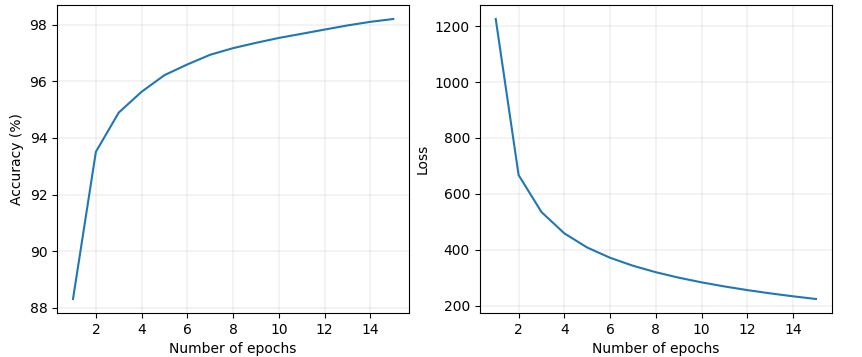
\includegraphics[scale=0.5]{./img/mnist.png}	
  \label{mnist}
  \caption{Accuracy plot of the MNIST dataset. The network is made up by one hidden layer with $50$ neurons, 
  and has been trained with a sigmoid activation function and a learning rate $\eta = 0.01$.}
\end{figure}
We can see that the network is able to learn the dataset and achieves very good accuracy values, just above
$98 \%$. This is confirmation that the framework actually works, and can be used to tackle real ploblems.
\newpage
\pagebreak

\section{Applying the neural network to the Higgs ML challenge}
\subsection{Preprocessing of the data}
The first step was to process the data, in order to make it more understandable for the network. \\ \\
The labels of the events are provided as chars, with $s$ indicating $signal$ events and $b$ representing 
$background$ events. These labels have been converted to integers, with $1$ indicating signal and $0$ 
indicating background. \\ \\
The dataset originally contains $818238$ events \cite{CERNOpenDataHiggsML}, but we can reduce this number drastically. In the 
documentation of the challenge is specified that when the value of a certain feature for an event can't be
calculated or is meaningless, it is given the value $-999.0$. This value was chosen because it is out of the 
range for all the features. So, in order to filter out incomplete events, we can discard all the events where
one or more feature have value $-999.0$. With this filter, the number of events goes from $818238$ to 
$223574$, thus making it much easier for the network to train on the dataset and greatly decreasing the 
execution times required by the training. \\
Now that we have cleaned the dataset, we proceed to divide it into the training, validation and test 
datasets. To do this we use the common rule of $80$/$10$/$10$, so $80\%$ of the events go in the training 
dataset, $10 \%$ in the validation dataset and the remaining $10 \%$ in the test dataset. \\ \\
Now we must prepare the feature values that we insert in the input layer of the network. We normalize the 
features with a standard scaler, so that we have mean $0$ and standard deviation $1$. This step is crucial
for this dataset, because the values of the features are very different between one another and span over 
very wide ranges, so if we didn't normalize these values we would need very high learning rates, high values 
for the weights and a lot of epochs in order to train the network. We first standardize the training dataset,
and then standardize the validation and test datasets with the mean and standard deviation calculated for
the training. It's important to normalize the data after the subdivision in training/validation/test, 
because otherwise we would normalize the training data with the test data, but they must be completely 
separate, so this would imply a contamination of the training dataset. \\ \\
As a last step, we could try to reduce the dimensionality using PCA. This isn't mandatory for this particular
dataset, because the number of features is already quite small ($d = 30$), but it's still interesing to 
perform a PCA to see how many of these features are needed to get a high residual value. \\
By performing PCA increasing the number of components we get the plot on the left in Fig. \ref{pca}, 
where it can be seen that to have a residual variance close to $0$ we need at least $25$ components, 
which means that for this dataset performing dimensionality reduction with PCA is not really a viable option.
\begin{figure}
  \centering
  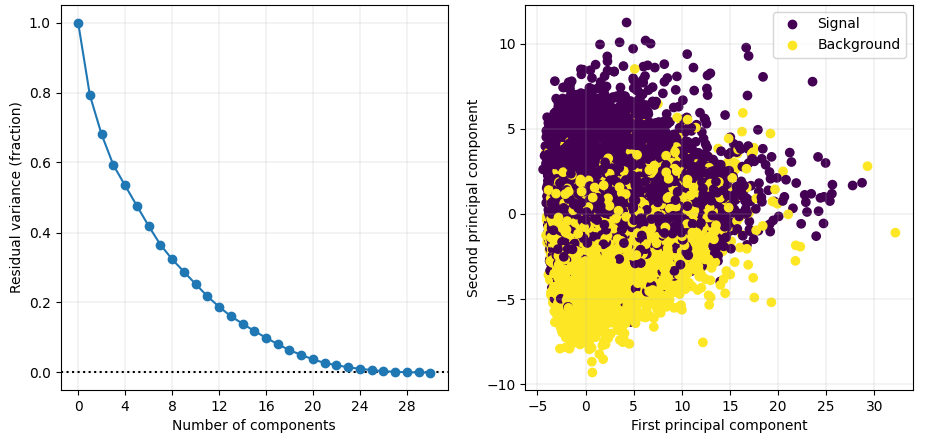
\includegraphics[scale=0.45]{./img/pca.png}
  \label{pca}
  \caption{On the left is the plot of the fractional residual variance obtained by perfoming a PCA on 
  the training dataset, as a function of the number of components. On the right is the scatter plot of 
  the two classes of events projected on the plane defined by the first two principal axis.}
\end{figure}
Considering the results obtained with the PCA, we try to plot the projection of the data onto the plane
defined by the eigenvectors of the first two principal components. Due to the low explained variance 
obtained with just two components, we would expect the two classes of points to overlap greatly, thus 
being impossible to separate, and this is in fact what we see in the right plot in Fig. \ref{pca}.

\subsection{Training, validation and testing}
For the challenge we used a fully connected neural network with $30$ neurons in the input layer, an hidden 
layer with $300$ nodes and a single neuron in the output layer, and is trained using a learning rate 
$\eta = 0.975$. \\
For classification problems with only two possible classes, like in this case, there are two alternatives: 
using one or two output neurons. These two possibilities are usually e\-qui\-va\-lent, but in this case 
we have opted for using a single neuron, because it has the simple advantage of decreasing the complexity 
of the calculations. \\ \\
To find the best architecture for the network and the optimal learning rate, we first do some tests to find 
the range of $\eta$ values which give the best accuracy. \\
We take learning rate values in the range $\eta \in [0.97, 0.99]$, where it was found that the accuracy
values were the highest, and for values in this range we train the network for several epochs, changing the
size of the hidden layer, and we observe the change in the accuracy values. \\
We take the learning rate values $\eta = 0.97, 0.975, 0.98, 0.985$ and train each neural network for $35$ 
epochs. The results are shown in the plots in Fig. \ref{accuracy_plots}, where it can be seen that the 
highest accuracy values are found for networks with between $300$ and $500$ neurons in the hidden layer
and trained with a learning rate between $\eta = 0.975$ and $\eta = 0.98$. \\
\begin{figure}
  \centering
  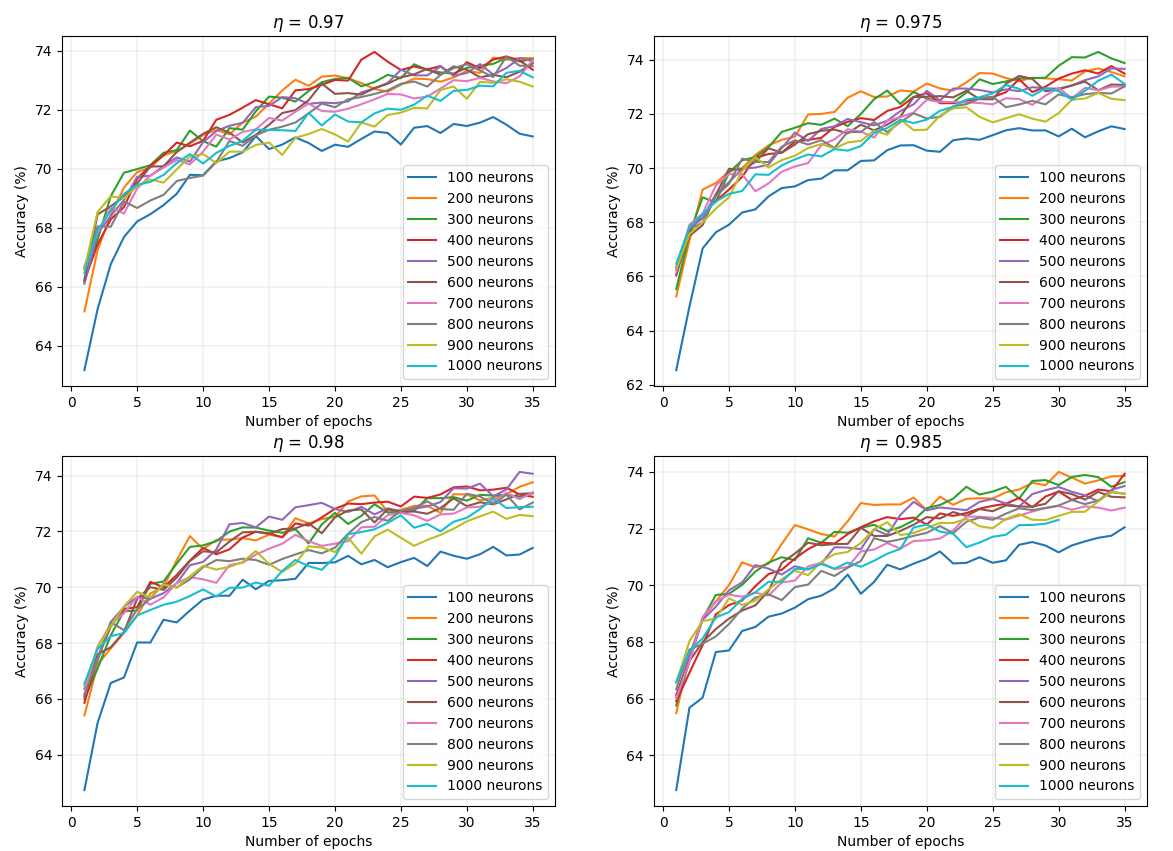
\includegraphics[scale=0.35]{./img/accuracy_plots.png}
  \label{accuracy_plots}
  \caption{Trends of accuracy on the training dataset in function of the number of the epochs. The measures
  have been repeated for different values of the learning rate, and for each one different sizes of the 
  hidden layer have been tested. It can be seen that the best accuracy is achieved with $\eta = 0.975$ and
  $N_h = 300$.}
\end{figure}
It is also interesting to observe, for the same values of $\eta$, the trend of the training loss as a 
function of the number of epochs. These trends are shown in the plots in Fig. \ref{training_loss}. We
can see that the values of the training loss are decreasing with the number of epochs, as they should, 
and the configurations $N_h = 300$, $N_h = 400$, $N_h = 500$ give some of the lowest values, for 
$\eta = 0.975$ and $\eta = 0.98$.
\begin{figure}
  \centering
  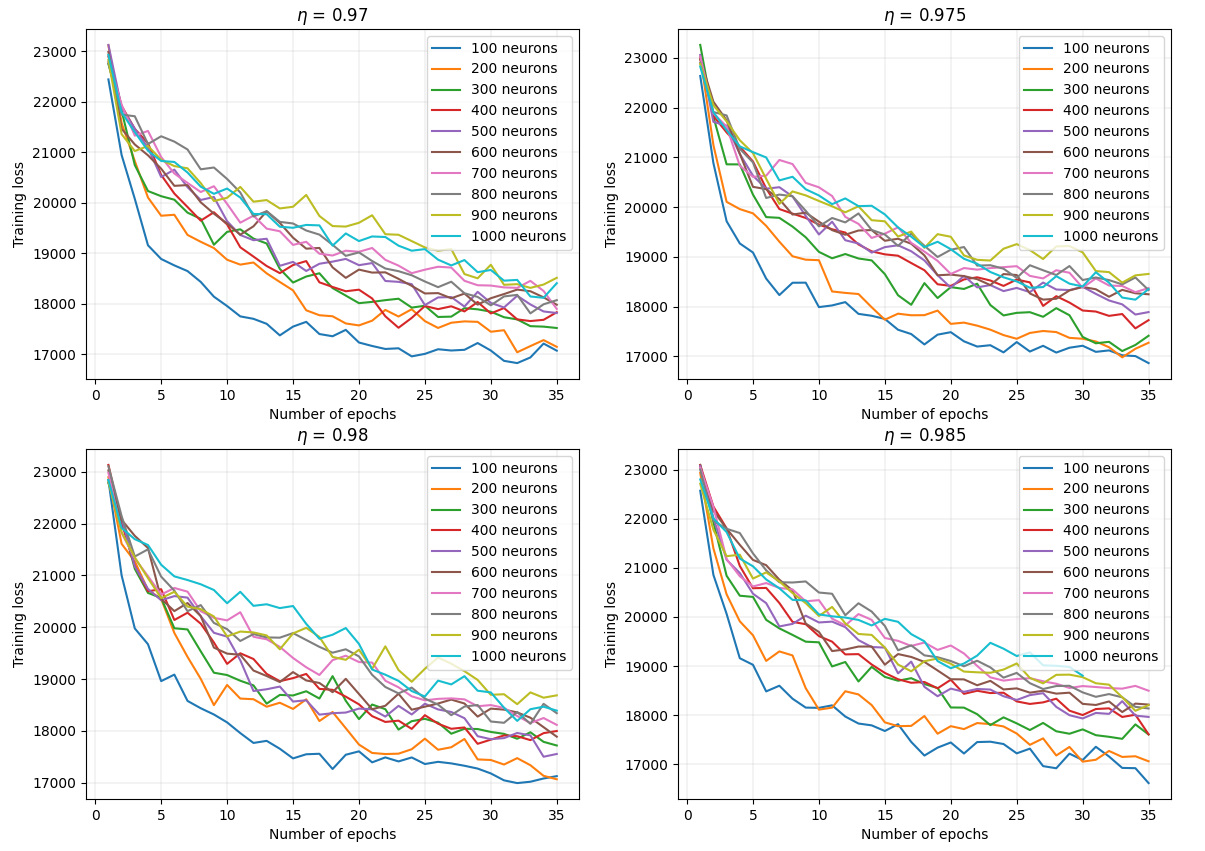
\includegraphics[scale=0.35]{./img/training_loss_plots.png}
  \label{training_loss}
  \caption{Trends of the training loss in function of the number of epochs. The measures have been repeated
  for different learning rates and changing the size of the hidden layer.}
\end{figure}
We thus decide to train and validate a neural network with $N_h = 300$ and using a learning rate 
$\eta = 0.975$. This choice is also motivated by the fact that, like we can see in Fig. \ref{accuracy_plots},
at the 35th epoch the accuracy is still in an increasing trend, which means that the network is not
overfitting the training data. \\
\tikzset{
  every neuron/.style={
    circle,
    draw,
    minimum size=0.7cm
  },
  neuron missing/.style={
    draw=none, 
    scale=3,
    text height=0.233cm,
    execute at begin node=\color{black}$\vdots$
  },
}

\begin{figure}
  \centering
  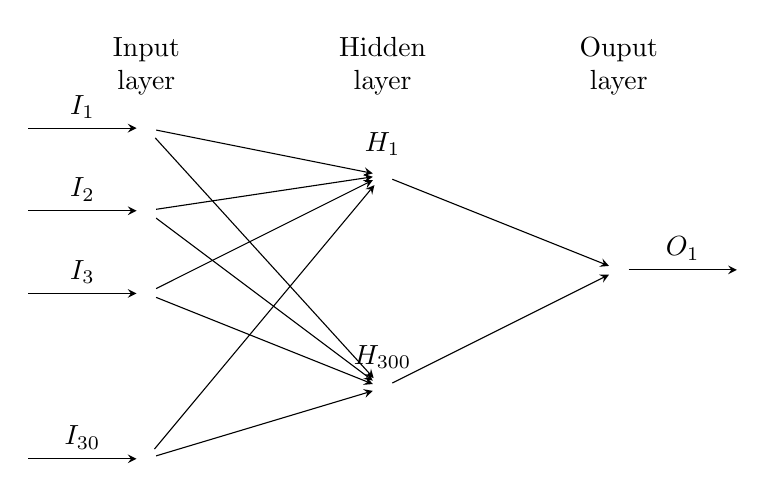
\begin{tikzpicture}[x=1.5cm, y=1.5cm, >=stealth]

  \foreach \m/\l [count=\y] in {1,2,3,missing,4}
	\node [every neuron/.try, neuron \m/.try] (input-\m) at (0,2.5-\y*0.7) {};

  \foreach \m [count=\y] in {1,missing,2}
	\node [every neuron/.try, neuron \m/.try ] (hidden-\m) at (2,2.3-\y*0.9) {};

  \foreach \m [count=\y] in {1}
	\node [every neuron/.try, neuron \m/.try ] (output-\m) at (4,1.6-\y) {};

  \foreach \l [count=\i] in {1,2,3,30}
	\draw [<-] (input-\i) -- ++(-1,0)
	  node [above, midway] {$I_{\l}$};

  \foreach \l [count=\i] in {1,300}
	\node [above] at (hidden-\i.north) {$H_{\l}$};

  \foreach \l [count=\i] in {1}
	\draw [->] (output-\i) -- ++(1,0)
	  node [above, midway] {$O_\l$};

  \foreach \i in {1,...,4}
	\foreach \j in {1,...,2}
	  \draw [->] (input-\i) -- (hidden-\j);

  \foreach \i in {1,...,2}
	\foreach \j in {1}
	  \draw [->] (hidden-\i) -- (output-\j);

  \foreach \l [count=\x from 0] in {Input, Hidden, Ouput}
	\node [align=center, above] at (\x*2,2) {\l \\ layer};

  \end{tikzpicture}
  \caption{Diagram of the neural network used for the challenge. The network has one hidden layer with 
  $400$ neurons and a single neuron in the output layer. One output neuron is enough since there are 
  only two categories, signal and background.}
\end{figure}
\noindent Now that we have found the best structure for the network, we repeat the training and perform 
the validation. \\
As can be seen in Fig. \ref{tv}, the accuracy values of the validation dataset are a lot more shaky and 
unstable, but this is very typical. By looking at the plots we see that the best accuracy values for both
training and validation are obtained with $22$ epochs. So, at this point the only thing left to do is to
repeat the training with $22$ epochs and test the result by executing a forward propagation on the test
dataset, and then calculate the accuracy. \\
The accuracy thus obtained on the test dataset is $79.5 \%$, which is a very good result, considering the 
simplicity of the network used for the task.
\begin{figure}
  \centering
  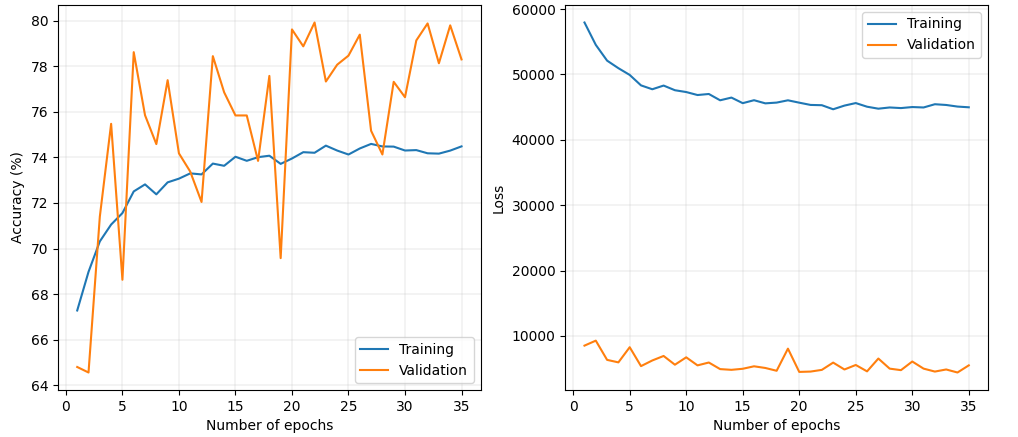
\includegraphics[scale=0.45]{./img/training_validation.png}
  \label{tv}
  \caption{On the left is the trend of the training accuracy in function of the number of epochs against the
  validation accuracy. On the right is the trend of the training loss against the validation loss.}
\end{figure}
\pagebreak

\section{Conclusions}
The neural network framework implemented in C++ has been tested on the MNIST dataset, achieving good values
of accuracy, which indicates that it works as expected and with reasonable execution times. \\
Then the framework has been applied to the Higgs ML challenge, whose goal is to classify a set of events
in signal and background, where the signal events consist of the decay of the Higgs boson, whereas 
background events consist of other decay processes with similar decay products, i.e. a pair of leptons. \\
This challenge has been tackled with a neural network consisting of a single hidden layer with $300$
neurons and a single output neuron, since the task is a classification problem. The network was then 
trained with a sigmoid activation function and a learning rate $\eta = 0.975$. \\
After the training and validation step, the optimal number of epochs was found to be $22$, so the network
was then trained again and tested on the test dataset, achieving an accuracy of $79.5 \%$. \\
This value of accuracy is quite good, especially considering that the winning solution of the challenge
used a bag of $70$ neural networks, made up by three hidden layers containing $600$ neurons each 
\cite{WinningModel}.
\pagebreak

\printbibliography

\end{document}
